\documentclass[12pt]{article}
\usepackage{sbc-template}
\usepackage{graphicx,url}
\usepackage{multicol}
\usepackage{subfigure}
\usepackage{color, soul}
%\usepackage[brazil]{babel}   
\usepackage[utf8]{inputenc}  

\sloppy

\title{Análise de Redes Sociais de Golfinhos e Atletas de Karatê}

\author{Rodrigo José Zonzin \inst{1} }


\address{Departamento de Computação -- Universidade Federal de São João del Rei
  (UFSJ)\\
    São João del Rei, Brasil
    }
\begin{document} 

\maketitle


\section{Introdução}
\section{Caracterização de Redes Reais}
O primeiro passo para análise das redes consistiu na obtenção de métricas descritivas dos grafos. Dessa maneira, a rede social de Golfinhos apresentou número de nós  $n = 62$, número de arestas $m = 159$, densidade  $D = 0.0841$ e coeficiente médio de clustering $\hat{c} = 0.2590$. Além disso, a rede apresenta distância média de $\hat{a} = 3.3569$. Por outro lado, a rede social de lutadores de Karatê apresentou $n = 34$, $m = 78$, densidade $D = 0.1390$, coeficiente médio de clustering $\hat{c} = 0.5706$ e distância média $\hat{a} = 2.4082$

Além disso, a figura \ref{metricas} resume a distribuição de algumas medidas de centralidade das redes em análise.  

\begin{figure}[h!]
    \centering
    \subfigure[Golfinhos]{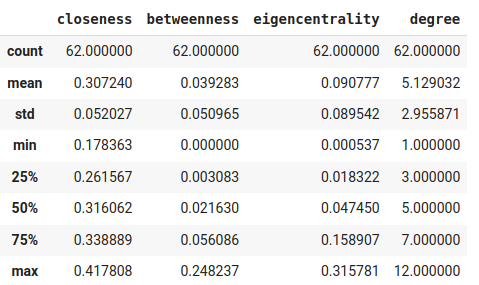
\includegraphics[width=0.45\linewidth]{rede_golfinho/metricas_redeGolfinhos.png}} 
    \qquad
    \subfigure[Karatê]{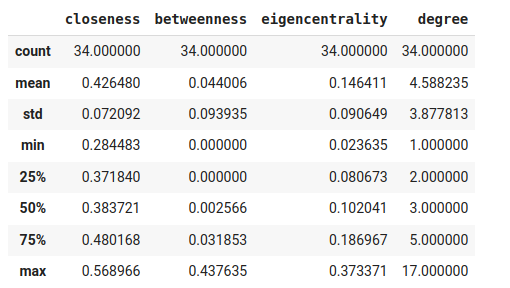
\includegraphics[width=0.45\linewidth]{rede_karate/metricas.png}}
    
    \caption{Métricas descritivas}
    \label{metricas}
\end{figure}

A Figura \ref{redes} apresenta o plot das redes. Os vértices estão discriminados,  conforme a centralidade por autovetor (Eigencentrality), por cor e tamanho.

\begin{figure}[h!]
    \centering
    \subfigure[Rede de Golfinhos]{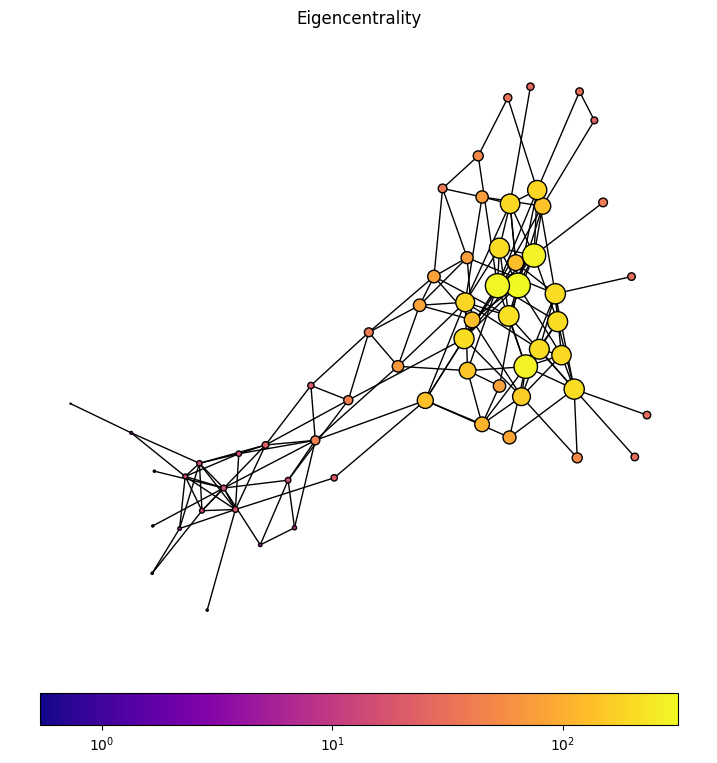
\includegraphics[width=0.45\linewidth]{rede_golfinho/plot_rede.png} \label{redegolfinho}}
    \qquad
    \subfigure[Rede de Karate]{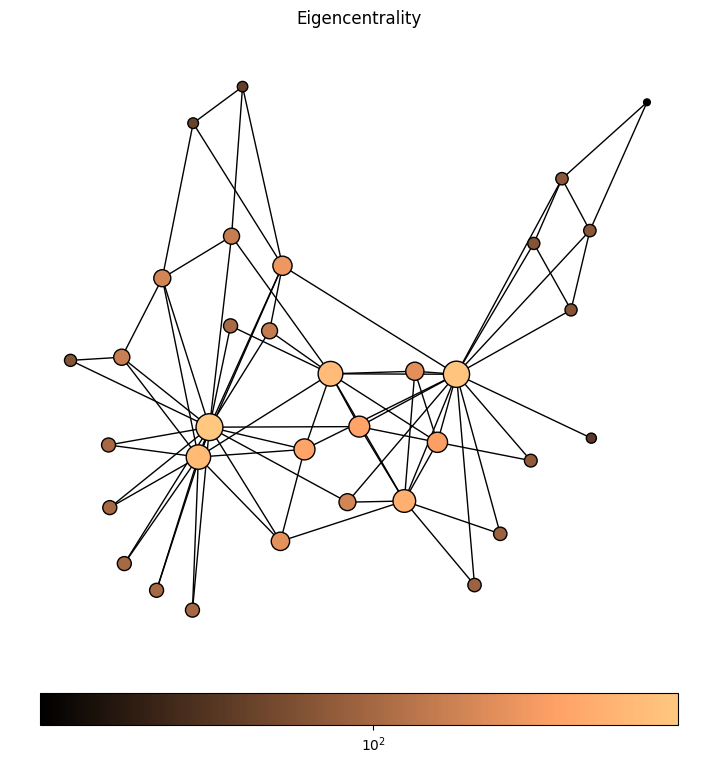
\includegraphics[width=0.45\linewidth]{rede_karate/plot_rede.png}\label{redekarate}}

    \caption{Redes em estudo}
    \label{redes}
\end{figure}


Além disso, a imagem a seguir apresenta a função de densidade de probabilidade e o histograma dos graus das rede, respectivamente. Por completude da análise, apresenta-se também a distribuição \textit{Log-Log} dos graus (Figura \ref{distribuicaoLogLog}). 

\begin{figure}[h!]
    \centering
    
    \subfigure[Golfinhos]{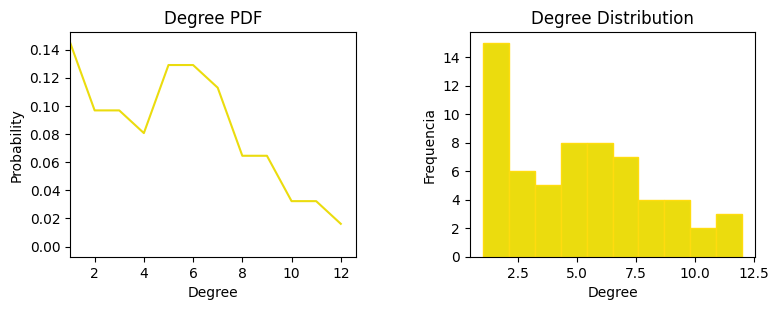
\includegraphics[width=0.7\linewidth]{rede_golfinho/degree_pdf.png}
    \label{pdfGolfinhos}}
    \qquad
    \subfigure[Karate]{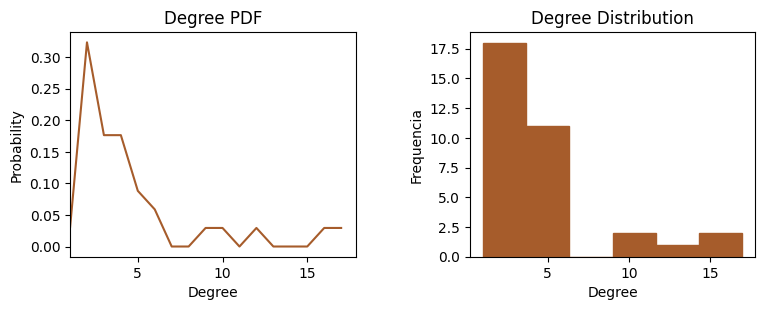
\includegraphics[width=0.7\linewidth]{rede_karate/histograma.png}
    \label{pdfKarate}}

    \caption{PDF e Histograma}
    \label{pdfHistogramaRedes}
\end{figure}

\begin{figure}[h!]
    \centering

    \subfigure[Golfinho]{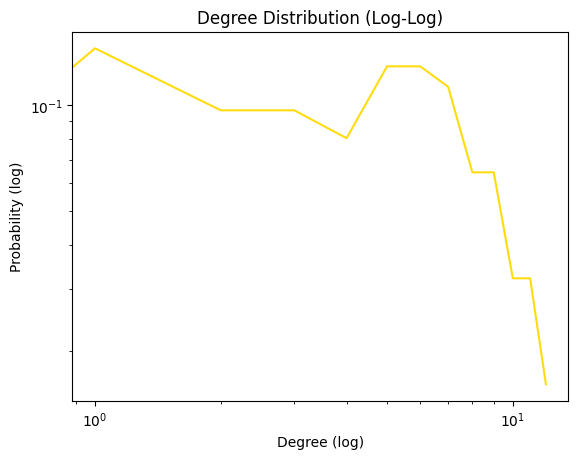
\includegraphics[width=0.3\linewidth]{rede_golfinho/degree_pdfLogLog.png}
    \label{logloggolfinho}}
    \qquad
    \subfigure[Karate]{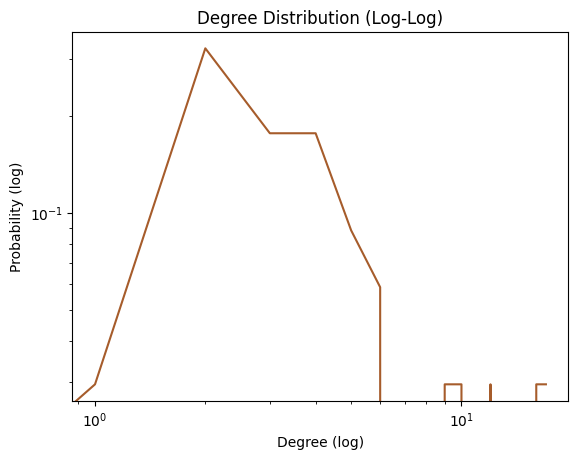
\includegraphics[width=0.3\linewidth]{rede_karate/logLog.png}\label{loglogkarate}}

    \caption{Distribuição Log-Log}
    \label{distribuicaoLogLog}

\end{figure}

\newpage

\section{Redes Erdos-Renyi}
Com o auxílio da biblioteca Networkx, obteve-se 9 redes Erdos-Renyi $G_{n, p}$ com $n = 1000$ e $p$ variando em 0.1 no intervalo $\left[ 0.1, 0.9\right]$. 

A figura \ref{metricasvsp} apresenta as medidas de Grau Médio, Clustering Médio, Densidade e Distância Média em função de $p$.  

\begin{figure}[h!]
    \centering
    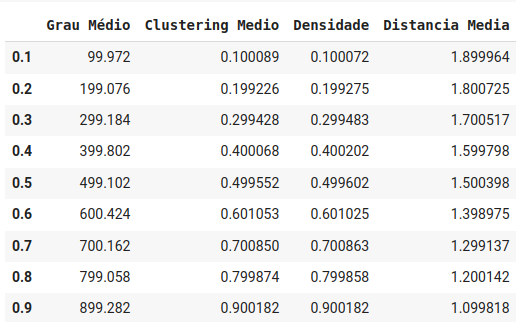
\includegraphics[width=0.5\linewidth]{valores_obtidos.png}
    \caption{Métricas vs $p$}
    \label{metricasvsp}
\end{figure}

Pode-se observar que a Densidade corresponde fielmente ao valor de $p$. Esse fato está em linha com a proposta do modelo $G_{n,p}$, que define a probabilidade de ocorrência das arestas. Para $p = 0$, nenhuma arestas é formada e o grafo apresentará $Densidade  = 0$. De forma oposta, se $p=1$, cada vértice está ligado a todos os demais, apresentando o número máximo de arestas possíveis $\frac{n(n-1)}{2}$ e, consequentemente, $Desnidade = 1$. 


De forma similar, o Clustering médio coincide com o valor de $p$. Sabe-se que o Clustering médio $\hat{C}$ é dado por: 
$$\hat{C} = \frac{1}{n}\sum_i^n c_i$$
como $c_i$ é constante $\forall i$, tem-se 

$$\hat{C} = \frac{1}{n}(nc_i)$$
$$\hat{C} = c_i$$
sabe-se que $c_i = p$ (a quantidade de arestas que cada vértice se liga é igual para todos os vértices e é dada por $p$)
$$\hat{C} = p$$

Os valores das métricas em função de $p$ indica que a Distância Média tem correlação negativa com $p$ ($\rho = -1$). De fato, sabe-se que a distância média é dada por 
$$I = \frac{log (n)}{log (<k> )} = \frac{log(n)}{log (2m/n)}$$

Como $m \propto p$, quanto maior for $p$, menor será a distância média.  

A figura \ref{plotredesdiferentesp} apresenta o plot da rede com o tamanho dos vértices proporcionais à centralidade por grau. Pode-se observar que a centralidade dos graus cresce uniformemente à medida que $p$ cresce. 

\begin{figure}[h!]
    \centering
    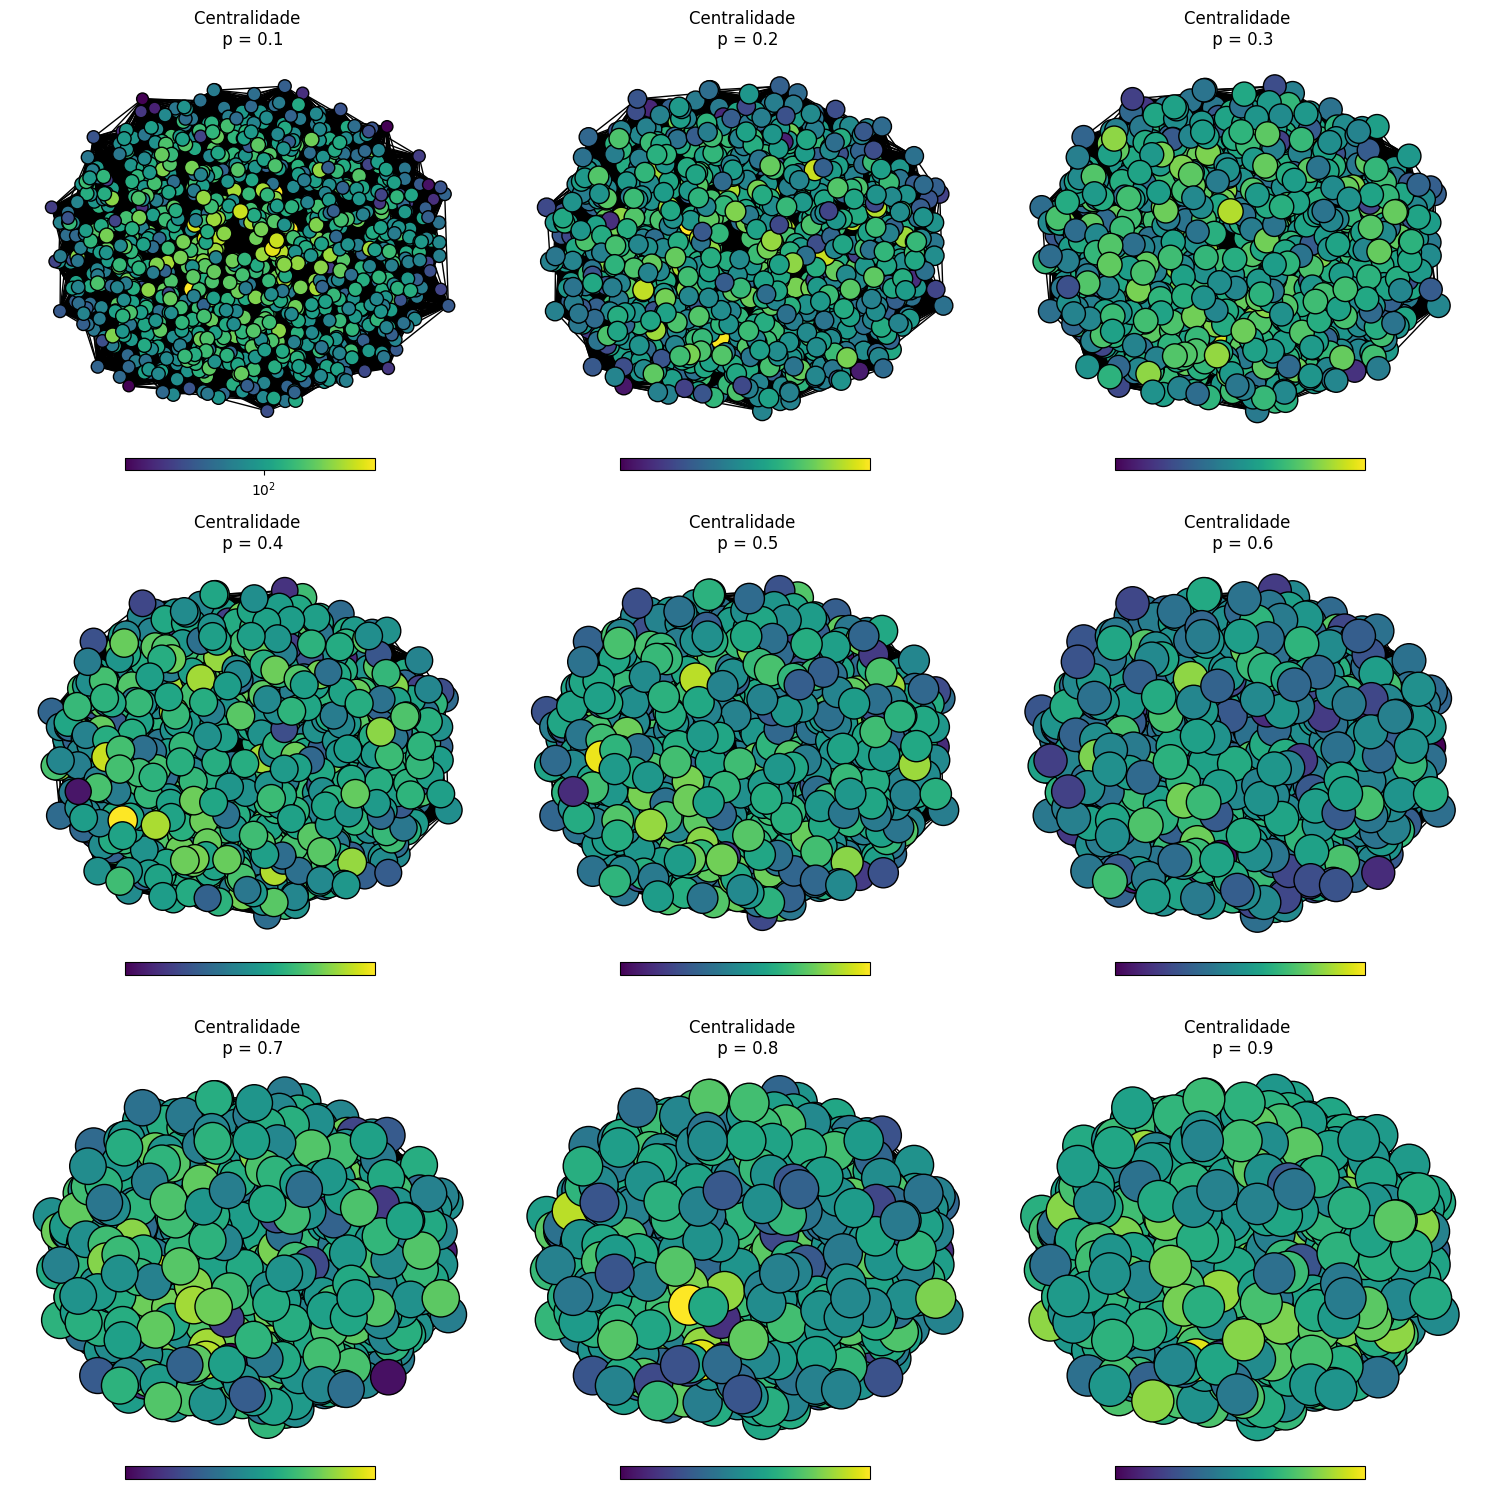
\includegraphics[width=0.9\linewidth]{plotRedes.png}
    \caption{Plot das redes para diferentes $p$}
    \label{plotredesdiferentesp}
\end{figure}



\bibliographystyle{sbc}
\bibliography{sbc-template}

\end{document}
